\documentclass{article}

\usepackage{amsmath, amsthm, amssymb, amsfonts}
\usepackage{thmtools}
\usepackage{graphicx}
\usepackage{setspace}
\usepackage{geometry}
\usepackage{float}
\usepackage{hyperref}
\usepackage[utf8]{inputenc}
\usepackage[english]{babel}
\usepackage{framed}
\usepackage[dvipsnames]{xcolor}
\usepackage{tcolorbox}

\hypersetup{
    colorlinks=true,
    linkcolor=black,
    citecolor=blue,
    urlcolor=cyan
}

\DeclareMathOperator{\spn}{span}

\graphicspath{{images/}}

\colorlet{LightGray}{White!90!Periwinkle}
\colorlet{LightOrange}{Orange!15}
\colorlet{LightGreen}{Green!15}
\colorlet{LightBlue}{Cyan!30}
\colorlet{LightRed}{Red!30}

\newcommand{\HRule}[1]{\rule{\linewidth}{#1}}

\declaretheoremstyle[
    name=Theorem,
    headpunct=\newline % Forces a newline after theorem title
]{thmsty}
\declaretheorem[style=thmsty,numberwithin=section]{theorem}
\tcolorboxenvironment{theorem}{colback=LightGray}

\declaretheoremstyle[
    name=Proposition,
    headpunct=\newline
]{prosty}
\declaretheorem[style=prosty,numberlike=theorem]{proposition}
\tcolorboxenvironment{proposition}{colback=LightOrange}

\declaretheoremstyle[
    name=Principle,
    headpunct=\newline
]{prcpsty}
\declaretheorem[style=prcpsty,numberlike=theorem]{principle}
\tcolorboxenvironment{principle}{colback=LightGreen}

\declaretheoremstyle[
    name=Example,
    headpunct=\newline
]{exsty}
\declaretheorem[style=exsty,numberlike=theorem]{example}
\tcolorboxenvironment{example}{colback=LightBlue}

\declaretheoremstyle[
    name=Definition,
    headpunct=\newline
]{defsty}
\declaretheorem[style=defsty,numberlike=theorem]{definition}
\tcolorboxenvironment{definition}{colback=LightRed}


\setstretch{1.2}
\geometry{
    textheight=9in,
    textwidth=5.5in,
    top=1in,
    headheight=12pt,
    headsep=25pt,
    footskip=30pt
}

% ------------------------------------------------------------------------------

\begin{document}

% ------------------------------------------------------------------------------
% Cover Page and ToC
% ------------------------------------------------------------------------------

\title{ \normalsize \textsc{}
		\\ [2.0cm]
		\HRule{1.5pt} \\
		\LARGE \textbf{\uppercase{Chapter 4: Orthogonality}
		\HRule{2.0pt} \\ [0.6cm] \LARGE{Introduction to Linear Algebra} \vspace*{10\baselineskip}}
		}
\date{}
\author{\textbf{Franklin Chen} \\ 
		Gilbert Strang \\
		Juanita High School \\
		26 Feburary 2025}

\maketitle
\newpage

\tableofcontents
\newpage

% ------------------------------------------------------------------------------

\section{Orthogonality of the Four Subspaces}
\begin{definition}[Orthogonal Subspaces]
    Subspaces $V$ and $W$ of a vector space are orthogonal if every vector in $V$ is perpendicular/orthogonal to every vector in $W$.
    
    \[\vec{v} \cdot \vec{w} = (\vec{v})^T \times \vec{w} = 0 \quad \forall \vec{v} \in V, \vec{w} \in W\]
\end{definition}

\begin{example}[Floors and Walls]
    Suppose you live in a rectangular room.
    The floor of your room (extended to infinity) is a subspace $F$.
    The line where two walls meet is a subspace $W$ (one-dimensional).
    $F$ and $W$ are orthogonal; every vector along $W$ is perpendicular to every vector along $F$.
    The origin $(0,0,0)$ is in the corner.
\end{example}

\begin{example}[Zero]
    If a vector is in two mutually orthogonal subspaces, then $\vec{v} \cdot \vec{v} = 0$.
    The only $\vec{v}$ that has this property is $\vec{0}$.
    $\vec{0}$ is the only vector that will be in two mutually orthgonal subspaces.
\end{example}

The crucial examples for Linear Algebra come from the fundamental subspaces.

\begin{theorem}
    The nullspace of $A$ is orthogonal to the row space of $A$.
    \begin{proof}
        Suppose $\vec{x}$ is in the nullspace of $A$.
        Then, $A \vec{x} = \vec{0}$.
        By the definitions of matrix-vector multiplication:

        \[A\vec{x} =
        \begin{bmatrix} % A
            \textrm{row 1} \\
            \textrm{row 2} \\
            \vdots \\
            \textrm{row $m$}
        \end{bmatrix}
        \begin{bmatrix} % x
            x_1 \\
            x_2 \\
            \vdots \\
            x_m 
        \end{bmatrix}
        =
        \begin{bmatrix} % Ax
            \textrm{row 1} \cdot \vec{x} \\
            \textrm{row 2} \cdot \vec{x} \\
            \vdots \\
            \textrm{row $m$} \cdot \vec{x}
        \end{bmatrix}
        =
        \vec{0}
        \]

        Because every cross product between the rows of $A$ and $\vec{x}$ equal zero, every row of $A$ is perpendicular to $\vec{x}$.
        This implies that the rows of $A$- the row space- and any vector in the nullspace of $A$ are mutually perpendicular.
        Thus, the nullspace of $A$ is orthogonal to the row space of $A$.
    \end{proof}
\end{theorem}

\begin{theorem}
    The left nullspace of $A$ (the nullspace of the row space) is orthogonal to the column space of $A$.
    \begin{proof}
        (Very similar proof to Theorem 1.4.)
        Suppose $\vec{y}$ is in the left nullspace.
        Then, $A^T \vec{y} = \vec{0}$. Taking the transpose, $(A^T \vec{y})^T = (\vec{y})^T A = (\vec{0})^T$.
        Expanding this out:

        \[(\vec{y})^T A =
        \begin{bmatrix} % (\vec{y})^T
            y_1& y_2& \cdots& y_n
        \end{bmatrix}
        \begin{bmatrix} % A
            \textrm{col 1}& \textrm{col 2}& \cdots& \textrm{col $n$}
        \end{bmatrix}
        \]
        \[
        =
        \begin{bmatrix} % (\vec{y})^T A
            \textrm{col 1} \cdot (\vec{y})^T & \textrm{col 2} \cdot (\vec{y})^T& \cdots& \textrm{col $n$} \cdot (\vec{y})^T
        \end{bmatrix}
        =
        (\vec{0})^T
        \]

        Every cross product between the cols of $A$ and $(\vec{y})^T$ equals zero, implying that the cols of $A$ and $(\vec{y})^T$ are mutually perpendicular.
        Thus, the left nullspace of $A$ is orthogonal to the column space of $A$.
    \end{proof}
\end{theorem}

Note that the fundamental subspaces are more than orthogonal: they are \textbf{orthogonal compliments} (which matter for some reason?)

\begin{definition}[Orthogonal Compliment]
    The orthogonal compliment of a subspace $V$ contains \textbf{all} vectors orthogonal to $V$.
    The orthogonal compliment is denoted $V^\perp$ ("v perp").
\end{definition}

By definition, the nullspace is the orthogonal complement of the row space, and similar with the left nullspace and the column space.
\textbf{Keep in mind what this implies}: every $\vec{x}$ orthogonal to the row space automatically satisfies $A\vec{x} = \vec{0}$, and every $\vec{y}$ orthogonal to the null space is automatically part of the row space.
$N(A)^\perp = R(A^T)$ and $R(A^T)^\perp = N(A)$!
Similar applies for the left nullspace and the column space.

This is all crystalised in the \textbf{Second Fundamental Theorem of Linear Algebra}:

\begin{theorem}[Second Fundamental Theorem of Linear Algebra]
    The nullspace is the orthogonal complement of the row space in $\mathbb{R}^n$.
    The left nullspace is the orthogonal complement of the col space in $\mathbb{R}^m$.
\end{theorem}

From what I understand, this implies that the nullspace plus the row space is equal to $\mathbb{R}^n$.
Thus, any input $\vec{x} \in \mathbb{R}^n$ can be broken down into the sum of a \textit{row space component} $\vec{x}_r$ and a \textit{null space component} $\vec{x}_n$.
So, for any $\vec{b} \in R(A)$:
\begin{enumerate}
    \item By the definition of the column space, there exists a vector $\vec{x} \in \mathbb{R}^n$ such that $A\vec{x} = \vec{b}$.
    \item Shown above, $\vec{x} = \vec{x}_r + \vec{x}_n$.
    \item $A\vec{x} = A(\vec{x}_r + \vec{x}_n) = A \vec{x}_r + \vec{0} = A \vec{x}_r = \vec{b}$ !
\end{enumerate}

Furthermore, Theorem 1.8 can be shown:

\begin{theorem}[Row Space and Col Space one-to-one mapping]
    For every vector $\vec{y}$ in the column space, there exists \textit{one and only one} vector $\vec{x}$ in the row space such that $A\vec{x} = \vec{y}$.

    \begin{proof}
        Suppose there exists $\vec{x'}$ in the row space such that $A\vec{x} = A\vec{x'}$.
        The difference $\vec{x} - \vec{x'}$ can be observed to be in the nullspace (maps to 0).
        By the additive property of subspaces, $\vec{x} - \vec{x'}$ is also part of the row space.
        As zero is the only vector that can be in two mutually orthogonal subspaces, this difference must equal zero.
        As such, $\vec{x} = \vec{x'}$.
    \end{proof}
\end{theorem}

If we "throw away" the nullspaces, we can see that \textit{there is always(?) an invertible matrix "hiding" within any matrix} because of this one-to-one mapping.

\begin{example}[Hidden Invertible Matrix]
    \[A =
    \begin{bmatrix}
        3& 0& 0& 0& 0 \\
        0& 5& 0& 0& 0 \\
        0& 0& 0& 0& 0   
    \end{bmatrix}
    \textrm{ contains }
    \begin{bmatrix}
        3& 0 \\
        0& 5
    \end{bmatrix}
    \]

    The hidden invertible matrix will always have size $r \times r$: both the row space and col space are of dimension $r$.
\end{example}

The following is quite useful, and is provided without proof:
\begin{theorem}[Linear Independence and Span]
    Any $n$ linearly independent vectors in $\mathbb{R}^n$ must span $\mathbb{R}^n$.
    Any $n$ vectors that span $\mathbb{R}^n$ must be linearly independent.
\end{theorem}

\newpage

\section{Projections}
\begin{definition}[Projection]
    The \textbf{projection} of some vector $\vec{b}$ onto a subspace $A$ is the vector $\vec{p}$ such that $\vec{p} \in \spn(A)$ and $|\vec{p} - \vec{b}|$ is minimized.
\end{definition}

\begin{example}[Projections as Components]
    Suppose $\vec{b} = (2,3,4)$.
    The projection of $\vec{b}$ onto the z-axis is the "shadow of $\vec{b}$ on the z-axis": $\vec{b}_z = (0,0,4)$.
    Similarly, the projection of $\vec{b}$ onto the xy-plane is the "shadow of $\vec{b}$ on the xy-plane": $\vec{b}_{xy} = (2, 3, 0)$.

    Such projections have matrices associated with them.
    Generally, the projections of a vector onto a line will have a rank one matrix associated, and a projection onto a plane a rank two matrix associated.
    Projection matricies should generally satisfy $\vec{p} = P \vec{b}$. For this example:

    \[P_{z} = \begin{bmatrix}
        0& 0& 0\\
        0& 0& 0\\
        0& 0& 1
    \end{bmatrix}\]

    \[P_{xy} = \begin{bmatrix}
        1& 0& 0\\
        0& 1& 0\\
        0& 0& 0
    \end{bmatrix}\]

    Generally, \textbf{we will be projecting vectors onto the column space of some arbitrary matrix $A$}.
    In this case, these matrices are nice because we're projecting onto the core axes and planes.
    Keep in mind, often, this projection will be much nastier.

    \[A_{z} =\begin{bmatrix}
        0\\
        0\\
        1
    \end{bmatrix}\]

    \[A_{xy} = \begin{bmatrix}
        1& 0\\
        0& 1\\
        0& 0\\
    \end{bmatrix}\]

\end{example}

\newpage

\subsection{Projection onto a Line}
\begin{figure}[htbp]
    \center
    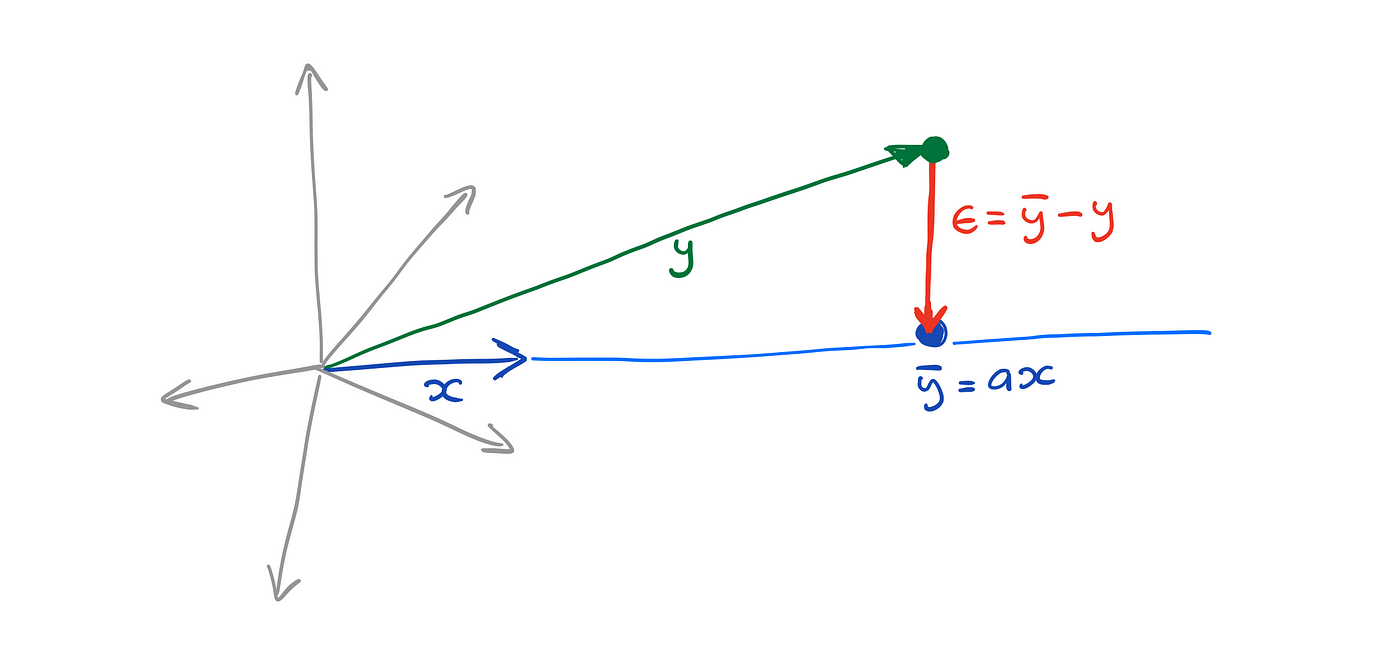
\includegraphics[scale=0.2]{projection.png}
    \caption{The projection of $\vec{y}$ onto $\vec{x}$, denoted $\bar{y}$. Ideally, we want to minimize $\epsilon = \bar{y} - \vec{y}$.}
\end{figure}

Suppose we are given two vectors $\vec{x}$ and $\vec{y}$ in $\mathbb{R}^m$, and we want to find the projection $\bar{y}$ on the line $\vec{x}$ such that $\vec{y}$ and its projection are as close as possible.
\textbf{The key is orthogonality}: the line connecting $\vec{y}$ and $\bar{y}$ ($\epsilon$) is \textit{perpendicular} to $\vec{x}$.

The projection is some multiple of $\vec{x}$: $\bar{y} = a \vec{x}$.
$\epsilon = \bar{y} - \vec{y} = a \vec{x} - \vec{y}$ is perpendicular to $\vec{x}$, so:

\[\vec{x} \cdot (a \vec{x} - \vec{y}) = 0\]

\[= a \vec{x} \cdot \vec{x} - \vec{y} \cdot \vec{x}\]

\[\implies a = \frac{\vec{x} \cdot \vec{y}}{\vec{x} \cdot \vec{x}} = \frac{(\vec{x})^T \vec{y}}{(\vec{x})^T \vec{x}}\]

\[\implies \bar{y} = a \vec{x} = \frac{(\vec{x})^T \vec{y}}{(\vec{x})^T \vec{x}} \vec{x}\]

This provides an explicit formula for the projection $\bar{y}$, without dealing with any nasty trig functions.
It is provided without proof that this equation for projection lines up with the traditional trigonometric way of finding projections.

The general \textbf{projection matrix} is also visible in this equation.
If $\bar{y} = a \vec{x} = P \vec{y}$, then, by rearranging the fraction (bring up $\vec{x}$ and put down $\vec{y}$):

\[P = \frac{\vec{x} (\vec{x})^T}{(\vec{x})^T \vec{x}}\]

$P$ is a column times row, so it is a $m \times m$ matrix \textit{of rank one} (as we are projecting onto a one-dimensional subspace: the line through $\vec{x}$).

Various remarks about $P$:
\begin{itemize}
    \item Because $P$ is defined using the \textit{line} through $\vec{x}$, only the \textbf{direction} of $\vec{x}$ matters: changing the magnitude of $\vec{x}$ changes nothing.
    \item $P^n = P$: projecting multiple times onto the same line does nothing.
    \item (?) The sum of the diagonal of $P$ equals 1.
    \item $I - P$ is a projection onto the line through $\epsilon$: the perpendicular subspace.
\end{itemize}

\subsection{Projection onto a Subspace}
Now, instead of projecting a vector $\vec{y}$ onto another vector $\vec{x}$, we want to project onto a \textbf{subspace}.
We want to find the "closest" vector to a target vector $\vec{b}$ within the subspace.
In other words: \textbf{find the combination of basis vectors $\bar{x}_1 \vec{a}_1 + \cdots + \bar{x}_n \vec{a}_n$ that is closest to the target vector}.

When $n = 1$, this is projection onto a line.
However, in general, we are projecting onto an linearly independent matrix $A$: we are looking for the particular $\vec{p} = A \bar{x}$, such that $\vec{p}$ is closest to $\vec{b}$.
We solve this problem in three steps: finding $\bar{x}$, finding the projection $\vec{p} = A \bar{x}$, and finding the matrix $P$.

Similar to the $n = 1$ case, \textbf{the key is in orthogonality}: the error vector $\vec{b} - A \bar{x}$ is \textit{perpendicular} to the column space of $A$. ($\vec{b} - A \bar{x}$ is in the left nullspace of $A$).
Mathematically:

\[\begin{matrix}
    (\vec{a}_1)^T (\vec{b} - A \bar{x}) = 0 \\
    \vdots \\
    (\vec{a}_n)^T (\vec{b} - A \bar{x} = 0)
\end{matrix}\]

The coefficents $(\vec{a}_n)^T$ can be extracted out as $A^T$.
Thus, the $n$ equations are exactly $A^T (\vec{b} - A \bar{x}) = \vec{0}$.
Or, in another form, $A^T A \bar{x} = A ^ T \vec{b}$.

This equation allows us to derive $\bar{x}$ as $\bar{x} = (A^T A) ^ {-1} A^T \vec{b}$.
From this, the projection of $\vec{b}$ onto the subspace is $\vec{p} = A \bar{x} = A (A^T A) ^ {-1} A^T \vec{b}$.
It can be observed that $P = A (A^T A) ^ {-1} A^T$.
It is provied without proof that this alligns with the formula derived for $n = 1$.

\subsubsection{Alternate Calculation for a projection}
From above, $A^T (\vec{b} - A \bar{x}) = \vec{0}$.
This implies that $\vec{b} - A \bar{x}$ is in the left nullspace.
Denoting the left nullspace matrix $A_{\perp}$, $\vec{b} - A \bar{x} = A_{\perp} \bar{y} \rightarrow \vec{b} = A \bar{x} + A_{\perp} \bar{y}$.
We can combine this into a segemented dot product:

\[
\begin{bmatrix} % matrix matrix
    A& A_{\perp}
\end{bmatrix}
\begin{bmatrix} % bar matrix
    \bar{x} \\
    \bar{y}
\end{bmatrix}
=
\vec{b}
\]

We can then use RREF to find $\bar{x}$, and calculate the projection as $A \bar{x}$.
This method also provides $\bar{y}$, which captures the part of $\vec{b}$ not captured by the projection: $A_{\perp} \bar{y}$.
(this can also be observed in the formula for $\vec{b}$ as the orthogonal component!)

So, to find the projection $\vec{p}$ from a vector $\vec{p}$ on a subspace $A$:
\begin{enumerate}
    \item Use RREF to find the basis of the nullspace of $A^T$. Use these as the columns for $A_{\perp}$.
    \item Use RREF to solve the segemented matrix equation for $\bar{x}$ and $\bar{y}$.
    \item Calculate $\vec{p} = A \bar{x}$. If needed, calculate the error as $A_{\perp} \bar{y}$.
\end{enumerate}




\subsection{random other things}
The matrix $A$ is rectangular: $A^-1$ doesn't exist.
Don't try to rearrange the projection matrix.

$A^T A$ is invertible, square, symmetric iif the columns of $A$ are linearly independent. there's a prooof but i'm too lazy to put it

\section{Least Squares Approximations}


\section{Orthogonal Bases and Gram-Schmidt}
\cite{ctan}

\newpage

\nocite{*}
\bibliographystyle{IEEEtran}
\bibliography{references.bib}


\end{document}